\section{Motivating Observations}
\label{section:motivation}
\paragraph{The optimal draft length is request-dependent.}
We first ask whether a single shared draft length can serve all requests well. To answer this, we run a study on 256 LongBench samples with prefix lengths in \([16\mathrm{k}, 20\mathrm{k}]\). For each request and each verification round, we record how many drafted tokens are accepted when drafting 20 tokens, over up to 1k generated tokens. Figure~\ref{fig:mob}(a) shows the per-request average accepted draft length. The distribution is broad, ranging from 2.56 to 20.00 with mean 11.51, indicating substantial heterogeneity, showing that different requests favor different draft lengths, and therefore a single shared draft length is inherently suboptimal.

\paragraph{The optimal draft length also changes over time within a request.}
Figure~\ref{fig:mob}(b) shows the number of accepted drafted tokens at each verification round for every request. Rows are sorted by each request's average accepted draft length in descending order to highlight cross-request heterogeneity. The apparent taper is a consequence of this sorting. Requests with higher average accepted draft lengths appear toward the top, commit more tokens per verification round, and therefore reach the final answer or generation-length cap in fewer rounds. Within individual rows, however, accepted draft length fluctuates substantially across verification rounds. Thus, neither a shared fixed draft length nor a fixed request-specific draft length is sufficient. Together with the cross-request heterogeneity in Figure~\ref{fig:mob}(a), this motivates per-request, step-level scheduling rather than synchronized batch-wide drafting and verification.

\begin{figure*}[t]
    \centering
    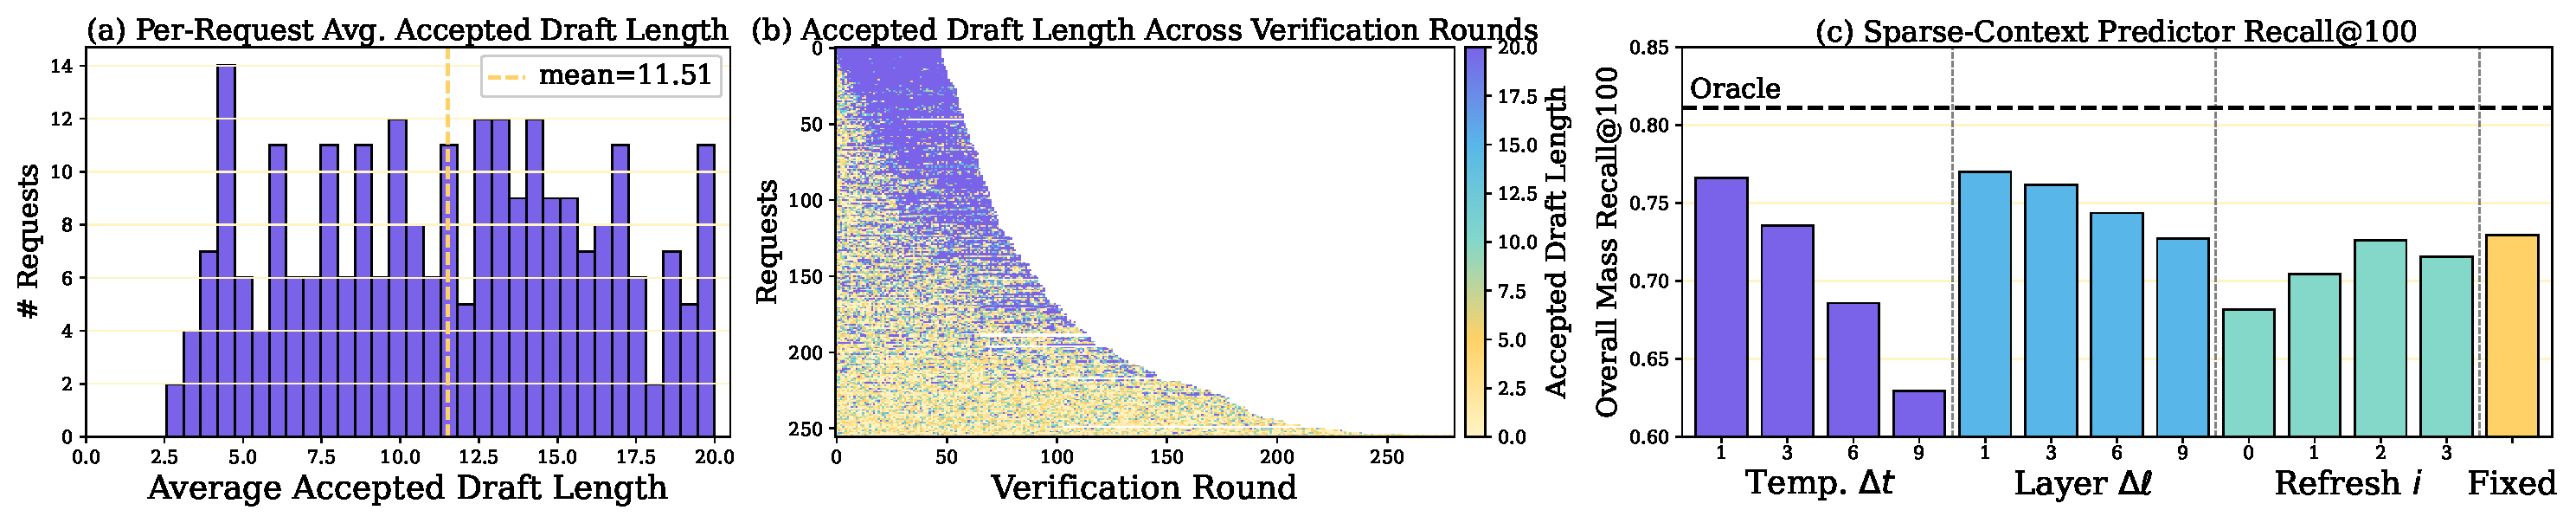
\includegraphics[width=\textwidth]{figs/mob.eps}
    \caption{(a) Average accepted draft length varies widely across requests. (b) Accepted length changes across verification rounds within each request. Rows are sorted by their mean in descending order, producing the aggregate taper; white cells occur after completion. (c) Sparse-context predictor recall for temporal, cross-layer, and single-refresh-layer sources. The fixed source uses the penultimate layer of the previous token.}
    \label{fig:mob}
\end{figure*}

\paragraph{Cross-layer signals are more stable than temporal reuse.}
\label{section:mob3}
Figure~\ref{fig:mob}(c) evaluates how well different attention-map sources predict the sparse context needed by a target token at a target layer. For each candidate source, we use its attention map to select the top-100 KV pages and measure the fraction of the target token/layer's total attention mass that falls on those pages, reported as overall mass recall@100. The oracle uses the target token/layer's own attention map to select the top-100 pages and therefore represents the best achievable recall under the same page budget.

The first group, Temp.~$\Delta t$, uses the same layer's attention map from earlier tokens to predict the current token. Recall decreases quickly as token lag $\Delta t$ grows, showing that attention maps from earlier draft tokens become stale during drafting. The second group, Layer~$\Delta \ell$, uses the attention map from exactly $\Delta \ell$ earlier layers of the same token. For example, with $\Delta \ell$$=$$1$, each target layer uses the attention map of its immediately preceding layer. Recall degrades much more slowly as $\Delta \ell$ increases than under temporal reuse, showing that nearby cross-layer signals are more stable predictors of the target sparse context. However, this comparison is primarily diagnostic, since using a fixed layer offset for every target layer would require multiple layer-specific refresh signals across the network.

\paragraph{A fixed late-layer source provides the best quality-overhead tradeoff.}
\label{section:mob4}
The third group, Refresh~$i$, evaluates a practical design with a single same-token refresh point. All layers through layer $i$ perform full attention, after which the attention map of layer $i$ is used to select sparse KV pages for the remaining layers. Moving the refresh point deeper can provide a stronger predictor, but directly increases the number of full-attention layers executed at every draft step. In Figure~\ref{fig:mob}(c), recall improves from refresh layers 0 to 2 and then changes little, indicating limited benefit from additional full-attention layers.

These observations motivate ASPIRE's fixed late-layer source from the previous token. The source is only one token old and comes from a late layer, combining the low temporal staleness of $\Delta t$$=$$1$ with a strong cross-layer signal. Unlike same-token Refresh~$i$, this design requires only a single full-attention layer per draft step while achieving comparable sparse-context recall.
